\documentclass[a4paper,12pt]{article}

% Packages for better formatting and functionalities
\usepackage[utf8]{inputenc}
\usepackage[english, greek]{babel}
\usepackage{amsmath}
\usepackage{graphicx}
\usepackage{hyperref}
\usepackage{geometry}
\usepackage{caption}
\usepackage{listings}
\geometry{a4paper, margin=1in}

% Title and Author
\title{Αναφορά Εργασίας: Ανάλυση Δεδομένων με \textlatin{Streamlit} και \textlatin{Docker}}
\author{Ευάγγελος Κωνσταντινίδης \textlatin{inf2021-113} \\
        Εμμανουήλ Μπιλιούρης \textlatin{inf2021-159} \\
        Φώτιος Σταματόπουλος \textlatin{inf2021-212}}
\date{\today}

\begin{document}

\selectlanguage{greek}

\maketitle

% Link to the app
\begin{center}
    \textbf{\textlatin{Link to the App}:} \href{https://softwaretechnology-b42qedritrsylcjthcxrvx.streamlit.app}{\textlatin{https://softwaretechnology-b42qedritrsylcjthcxrvx.streamlit.app}}
\end{center}

\begin{center}
    \textbf{\textlatin{Link to the Github rep}:} \href{https://github.com/ManosBiliouris/Texnologia_Logismikou/tree/master}{\textlatin{Github}}
\end{center}

\begin{abstract}
Η παρούσα αναφορά περιγράφει την ανάπτυξη μιας διαδικτυακής εφαρμογής για την ανάλυση δεδομένων χρησιμοποιώντας \textlatin{streamlit} και \textlatin{Docker}. Η αναφορά περιλαμβάνει λεπτομέρειες του σχεδιασμού της εφαρμογής, την υλοποίηση, τα αποτελέσματα των αναλύσεων, τα συμπεράσματα, καθώς και την περιγραφή της συνεισφοράς κάθε μέλους της ομάδας.
\end{abstract}

\tableofcontents
\newpage

\section{Εισαγωγή}
\label{sec:intro}
Η εργασία αυτή επικεντρώνεται στην ανάπτυξη μιας διαδικτυακής εφαρμογής ανάλυσης δεδομένων. Στόχος της είναι η εύκολη χρήση εργαλείων μηχανικής μάθησης και η παρουσίαση των αποτελεσμάτων με έναν κατανοητό τρόπο. Η εφαρμογή χρησιμοποιεί \textlatin{Streamlit} για τη δημιουργία του διεπαφής χρήστη και \textlatin{Docker} για την εξασφάλιση συνέπειας στο περιβάλλον εκτέλεσης. \textbf{Η εργασία αυτη έχει δοκιμαστεί πάνω σε 2 πολύ διάσημα \textlatin{CSV files}, το \textlatin{Iris dataset} και το \textlatin{Wine Quality dataset}}.

\section{Σχεδιασμός της Εφαρμογής}
\label{sec:design}
Η εφαρμογή αποτελείται από τις εξής βασικές ενότητες:
\begin{itemize}
    \item Ανέβασμα αρχείου δεδομένων
    \item Οπτικοποίηση δεδομένων σε 2 διαστάσεις (\textlatin{PCA}, \textlatin{t-SNE}, \textlatin{EDA})
    \item Αλγόριθμοι κατηγοριοποίησης (\textlatin{KNeighborsClassifier}, \textlatin{RandomForestClassifier})
    \item Αλγόριθμοι ομαδοποίησης (\textlatin{KMeans}, \textlatin{Agglomerative Clustering})
    \item Παρουσίαση αποτελεσμάτων και συγκρίσεων
\end{itemize}
Ο σχεδιασμός περιλαμβάνει επίσης τη χρήση \textlatin{Docker} για τη δημιουργία ενός περιβάλλοντος εκτέλεσης που διασφαλίζει τη συμβατότητα και την επαναληψιμότητα.

\section{Υλοποίηση}

\subsection{Ανέβασμα αρχείου δεδομένων}
Η εφαρμογή ξεκινά με την παροχή της δυνατότητας στους χρήστες να ανεβάσουν τα αρχεία τους. Χρησιμοποιούμε την εντολή \textlatin{"st.fileuploader"} για να επιτρέψουμε το ανέβασμα αρχείων.

\subsection{Οπτικοποίηση δεδομένων}
Η εφαρμογή παρέχει εργαλεία για την οπτικοποίηση των δεδομένων σε 2 διαστάσεις χρησιμοποιώντας τις μεθόδους \textlatin{PCA} και \textlatin{t-SNE}. Επιπλέον, προσφέρονται περιγραφικές στατιστικές αναλύσεις (\textlatin{EDA}).

\subsection{Αλγόριθμοι κατηγοριοποίησης}
Χρησιμοποιούνται οι αλγόριθμοι \textlatin{KNeighborsClassifier} και \textlatin{RandomForestClassifier} για την κατηγοριοποίηση των δεδομένων. Τα αποτελέσματα αξιολογούνται και συγκρίνονται με βάση την ακρίβεια και τον πίνακα σύγχυσης.

\subsection{Αλγόριθμοι ομαδοποίησης}
Η εφαρμογή χρησιμοποιεί τους αλγόριθμους \textlatin{KMeans} και \textlatin{Agglomerative Clustering} για την ομαδοποίηση των δεδομένων. Τα αποτελέσματα αξιολογούνται και συγκρίνονται με βάση το \textlatin{Silhouette Score}.

\subsection{Χρήση \textlatin{Docker}}
Η υλοποίηση της εφαρμογής σε \textlatin{Docker} επιτρέπει την εκτέλεση της σε οποιοδήποτε περιβάλλον με συνέπεια. Η διαδικασία περιλαμβάνει τη δημιουργία ενός \textlatin{Dockerfile} και την εγκατάσταση των απαραίτητων βιβλιοθηκών.

\section{Αποτελέσματα Κατηγοριοποίησης}
\begin{figure}[h!]
\centering
\includegraphics[width=0.9\textwidth]{APOTELESMA1.JPG}
\caption{Αποτελέσματα κατηγοριοποίησης χρησιμοποιώντας \textlatin{KNeighborsClassifier} και \textlatin{RandomForestClassifier}. Φαίνεται οτι η εφαρμογή υπολογίζει τον \textlatin{RandomForestClassifier} πιο αποδοτικό }
\end{figure}

\subsection{Αποτελέσματα Ομαδοποίησης}
\begin{figure}[h!]
\centering
\includegraphics[width=0.7\textwidth]{APOTELESMA2.JPG}
\caption{Αποτελέσματα ομαδοποίησης χρησιμοποιώντας \textlatin{KMeans} και \textlatin{Agglomerative Clustering}. Φαίνεται οτι η εφαρμογή υπολογίζει τον \textlatin{KMeans} πιο αποδοτικό}
\end{figure}

\section{Συμπεράσματα}
\label{sec:conclusion}
Η παρούσα εφαρμογή προσφέρει μια ολοκληρωμένη λύση για την ανάλυση δεδομένων με χρήση τεχνικών μηχανικής μάθησης. Η χρήση του \textlatin{Streamlit} για τη δημιουργία του διεπαφής χρήστη και του \textlatin{Docker} για τη διασφάλιση συνέπειας στο περιβάλλον εκτέλεσης είναι δύο βασικά πλεονεκτήματα της εφαρμογής.

Τα αποτελέσματα έδειξαν ότι κατά την εκτέλεση του dataset \textlatin{IRIS}, ο \textlatin{RandomForestClassifier} ήταν ο πιο γρήγορος αλγόριθμος κατηγοριοποίησης και ο \textlatin{KMeans} ήταν ο πιο γρήγορος αλγόριθμος ομαδοποίησης.

\section{Συνεισφορά Μελών Ομάδας}
\label{sec:contribution}
Η συνεισφορά κάθε μέλους της ομάδας περιγράφεται ως εξής:
\begin{itemize}
    \item Εύαγγελος Κωνσταντινίδης \textlatin{(github vag4me)}: Ανάπτυξη της εφαρμογής, Κύκλος Ζωής Έκδοσης Λογισμικού
    \item Εμμανουήλ Μπιλιούρης \textlatin{(github ManosBiliouris)}: Dockeration, Βοήθεια στην ανάπτυξη εφαρμογής.
    \item Φώτιος Σταματόπουλος \textlatin{(github FOTAKLAS)}: UML, Βοήθεια στην ανάπτυξη εφαρμογής.
\end{itemize}

\section{UML Διαγράμματα}
\label{sec:uml}

\subsection{Διάγραμμα Συστατικών}
Το ακόλουθο διάγραμμα συστατικών απεικονίζει την αρχιτεκτονική της εφαρμογής.

\begin{figure}[h!]
\centering
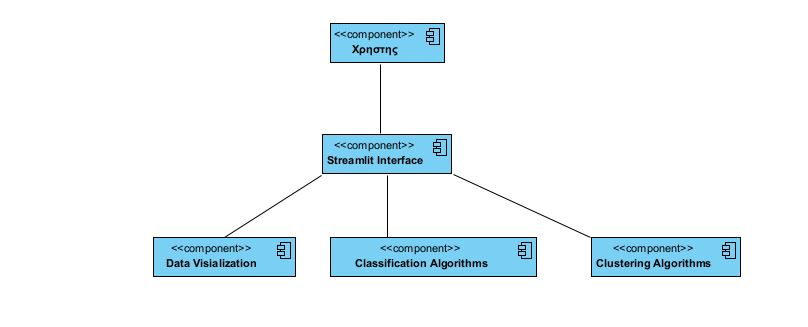
\includegraphics[width=0.8\textwidth]{UML2.JPG}
\caption{Διάγραμμα Συστατικών της αρχιτεκτονικής της εφαρμογής}
\label{fig:component}
\end{figure}

\subsection{Διάγραμμα Περιπτώσεων Χρήσης}
Το ακόλουθο διάγραμμα περιπτώσεων χρήσης απεικονίζει τις κύριες λειτουργίες της εφαρμογής και τις αλληλεπιδράσεις με τον χρήστη.

\begin{figure}[h!]
\centering
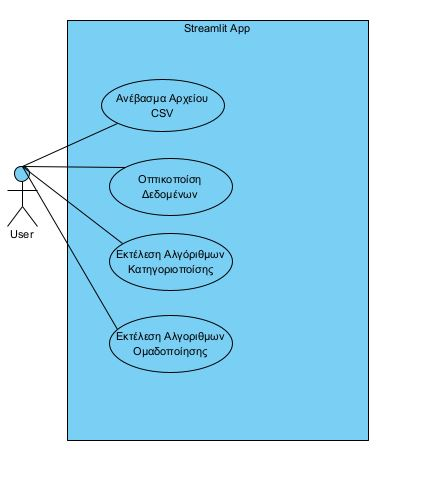
\includegraphics[width=0.8\textwidth]{UML1.JPG}
\caption{Διάγραμμα Περιπτώσεων Χρήσης της εφαρμογής}
\label{fig:usecase}
\end{figure}

\end{document}
